\begin{transitionframe}{Images/Transitions/CartoucheThutmosisReverse(WaltersArtMuseum)(PublicDomain)}{black} \centering
\textbf{Embedding Modal Logic into Higher-Order Logic}
\end{transitionframe}

\begin{frame}{Embedding QML in HOL} \large

\hskip-1em Challenge: \hfill No provers for \emph{Higher-order
  Quantified Modal
  Logic\/} (\textcolor{red}{QML}) \\[1em]

\hskip-1em Our solution: \hfill Embedding in \emph{Higher-order Classical
  Logic\/} (\textcolor{blue}{HOL}) \\
\, \hfill Then use existing \textcolor{blue}{HOL} theorem provers for reasoning in \textcolor{red}{QML} \\
\,\hfill {\small [Benzm\"ullerPaulson, Logica Universalis, 2013]}
\\[2em]

\hskip-1em Previous empirical findings:  \\[.5em]
\,\hfill Embedding of  \emph{First-order Modal Logic} in HOL works well 

\,\hfill {\small [Benzm\"ullerOttenRaths, ECAI, 2012]} \\
\,\hfill {\small [Benzm\"uller, LPAR, 2013]}
\end{frame}



\begin{frame}{Embedding QML in HOL} \large

\hskip-1em\textcolor{red}{QML} \hfill
$\begin{array}{lll}\textcolor{red}{\varphi,\psi} & ::= &
  \textcolor{red}{\ldots}  \mid \textcolor{red}{\neg
    \varphi} \mid \textcolor{red}{\varphi \wedge \psi} \mid
  \textcolor{red}{\varphi \imp \psi}  \mid \textcolor{red}{\Box
    \varphi} \mid \textcolor{red}{\Diamond \varphi}  \mid
  \textcolor{red}{\forall {x}\, \varphi} \mid
  \textcolor{red}{\exists {x}\, \varphi} 
\mid \textcolor{red}{\forall {P}\, \varphi} \end{array}$ \\[1em]


\begin{itemize}
\item Kripke style semantics (possible world semantics)\\[2em]
\end{itemize}



\hskip-1em\textcolor{blue}{HOL}\hfill 
$\begin{array}{lll}
\textcolor{blue}{s,t} & ::= & \textcolor{blue}{C}  \mid
\textcolor{blue}{x \mid \lambda{x} s} \mid \textcolor{blue}{s\, t}
\mid \textcolor{blue}{\neg s} \mid \textcolor{blue}{s \vee t} \mid
\textcolor{blue}{\forall {x}\, t} 
\end{array}$ \\[1em]

\begin{itemize}
\item various theorem provers exist \\[.5em]
  \quad interactive: \hfill Isabelle/HOL, HOL4, Hol Light, Coq/HOL, PVS,
  \ldots \\[.5em]
  \quad automated: \hfill TPS, LEO-II, Satallax, Nitpick, Isabelle/HOL, \ldots \\
\end{itemize}


\end{frame}


\begin{frame}{Embedding QML in HOL}\large

\hskip-1em\textcolor{red}{QML} \hfill
$\begin{array}{lll}\textcolor{red}{\varphi,\psi} & ::= &
  \textcolor{red}{\ldots}  \mid \textcolor{red}{\neg
    \varphi} \mid \textcolor{red}{\varphi \wedge \psi} \mid
  \textcolor{red}{\varphi \imp \psi}  \mid \textcolor{red}{\Box
    \varphi} \mid \textcolor{red}{\Diamond \varphi}  \mid
  \textcolor{red}{\forall {x}\, \varphi} \mid
  \textcolor{red}{\exists {x}\, \varphi} 
\mid \textcolor{red}{\forall {P}\, \varphi} \end{array}$ \\[1em]

\hskip-1em\textcolor{blue}{HOL}\hfill 
$\begin{array}{lll}
\textcolor{blue}{s,t} & ::= & \textcolor{blue}{C}  \mid
\textcolor{blue}{x \mid \lambda{x} s} \mid \textcolor{blue}{s\, t}
\mid \textcolor{blue}{\neg s} \mid \textcolor{blue}{s \vee t} \mid
\textcolor{blue}{\forall {x}\, t} 
\end{array}$ \\[1em]

\pause

\hskip-1em\textcolor{red}{QML} in \textcolor{blue}{HOL}: \quad \textcolor{red}{QML}
formulas $\textcolor{red}{\varphi}$ are mapped to
\textcolor{blue}{HOL} predicates $\textcolor{red}{\varphi_{\worldtype\typearrow o}}$

\begin{center}
\fcolorbox{blue}{white}{
$\begin{array}{lcl} 
    \textcolor{red}{\mnot} & = & \textcolor{blue}{
      \lambda{\varphi_{\worldtype\typearrow o}}\lambda{w_\worldtype}\neg \varphi w} \\ 
    \textcolor{red}{\mand} & = & \textcolor{blue}{ 
      \lambda{\varphi_{\worldtype\typearrow o}}
      \lambda{\psi_{\worldtype\typearrow o}} \lambda{w_\worldtype}
      (\varphi w \wedge \psi w)} \\ 
    \textcolor{red}{\imp} & = & \textcolor{blue}{ 
      \lambda{\varphi_{\worldtype\typearrow o}}
      \lambda{\psi_{\worldtype\typearrow o}} \lambda{w_\worldtype}
      (\neg \varphi w \vee \psi w)} \\ 
    \textcolor{red}{\forall} & = & \textcolor{blue}{ 
      \lambda{h_{\gamma\typearrow(\worldtype \typearrow o)}}
      \lambda{w_\worldtype} \forall {d_\gamma} \, h d w} \\
    \textcolor{red}{\exists} & = & \textcolor{blue}{ 
      \lambda{h_{\gamma\typearrow(\worldtype \typearrow o)}}
      \lambda{w_\worldtype} \exists {d_\gamma} \, h d w} \\
    \\
    \textcolor{red}{\Box} & = & \textcolor{blue}{ 
      \lambda{\varphi_{\worldtype\typearrow o}} \lambda{w_\worldtype}
      \forall {u_\worldtype}\, (\neg r w u \vee
      \varphi u)} \\ 
    \textcolor{red}{\Diamond} & = & \textcolor{blue}{ 
      \lambda{\varphi_{\worldtype\typearrow o}} \lambda{w_\worldtype}
      \exists {u_\worldtype}\, (r w u \wedge
      \varphi u)} \\ 
    \\
    \text{\textcolor{brown}{valid}} & = & \textcolor{blue}{
        \lambda{\varphi_{\worldtype\typearrow o}} \all{w_\worldtype}
        \varphi w}
\end{array}$
}  \quad \textcolor{blue}{Ax} 
\vskip1em
\end{center}

\pause

\quad The equations in \textcolor{blue}{Ax} are given as axioms to the \textcolor{blue}{HOL} provers! \\


\end{frame}



\begin{frame}{Embedding QML in HOL} \large

\hskip-1em Example \\[.5em]

 \textcolor{red}{QML} formula  \hfill \textcolor{red}{$\Diamond \exists x G(x)$}

\pause 

 \textcolor{red}{QML} formula in \textcolor{blue}{HOL}  \hfill $\text{\textcolor{brown}{valid}}\, \textcolor{red}{(\Diamond \exists x G(x))_{\worldtype\typearrow o}}$

\pause

expansion, $\beta\eta$-conversion \hfill $\textcolor{blue}{\forall
  w_\worldtype\textcolor{red}{(\Diamond \exists x
    G(x))_{\worldtype\typearrow o}}\, w}$ 

\pause

expansion, $\beta\eta$-conversion \hfill $\textcolor{blue}{\forall
  w_\worldtype \exists {u_\worldtype} (r w u \wedge
      \textcolor{red}{(\exists x G(x))_{\worldtype\typearrow o}} u)}$ 

% expansion, $\beta\eta$-conversion \hfill $\textcolor{blue}{\forall
%   w_\worldtype \exists {u_\worldtype} (r w u \wedge
%       \exists x \textcolor{red}{G(x)_{\worldtype\typearrow o}} u)}$ 

\pause

expansion, $\beta\eta$-conversion \hfill $\textcolor{blue}{\forall
  w_\worldtype \exists {u_\worldtype} (r w u \wedge
      \exists x G x u)}$ \\[1em]

\pause

\vfill
\begin{block}{What are we doing?}
\vskip.5em
In order to prove that $\textcolor{red}{\varphi}$ is valid in \textcolor{red}{QML}, \\
--> we instead prove that 
$\text{\textcolor{brown}{valid}}\,
\textcolor{red}{\varphi_{\worldtype\typearrow o}}$ can be derived
from \textcolor{blue}{Ax} in \textcolor{blue}{HOL}. \\[1em]

This can be done with interactive or automated \textcolor{blue}{HOL} theorem provers.
\end{block}
\pause
\vfill
\hskip-1em Expansion: \hfill user or prover may flexibly choose expansion depth \\[.5em]

\end{frame}


\begin{transitionframe}{Images/Transitions/GodComputerC}{black}
\textbf{
\quad Automated Proof Search and Consistency Check \hfill  \\
}
\end{transitionframe}


\begin{frame}{Automated Theorem Provers and Model Finders for HOL}
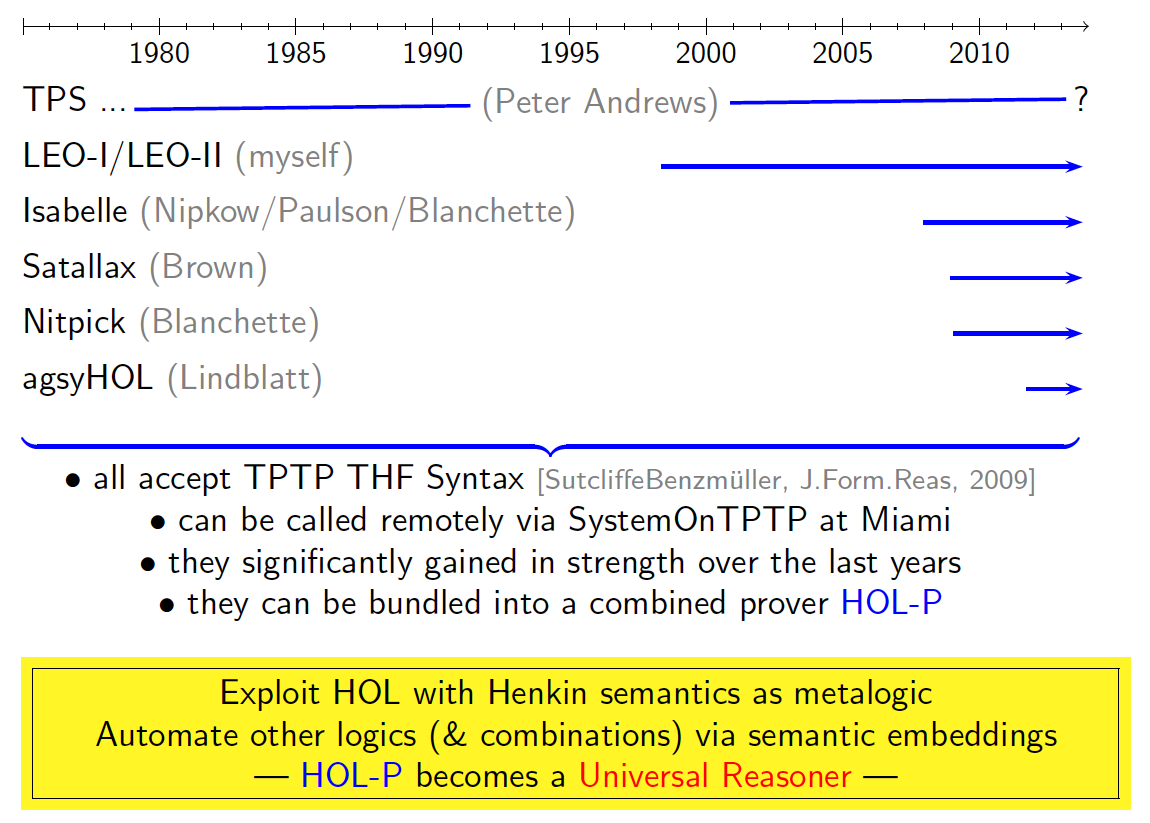
\includegraphics[width=1.05\textwidth]{Images/HOLProversGrab}
\end{frame}


\begin{frame}{Proof Automation and Consistency Checking} \large
\colorbox{gray}{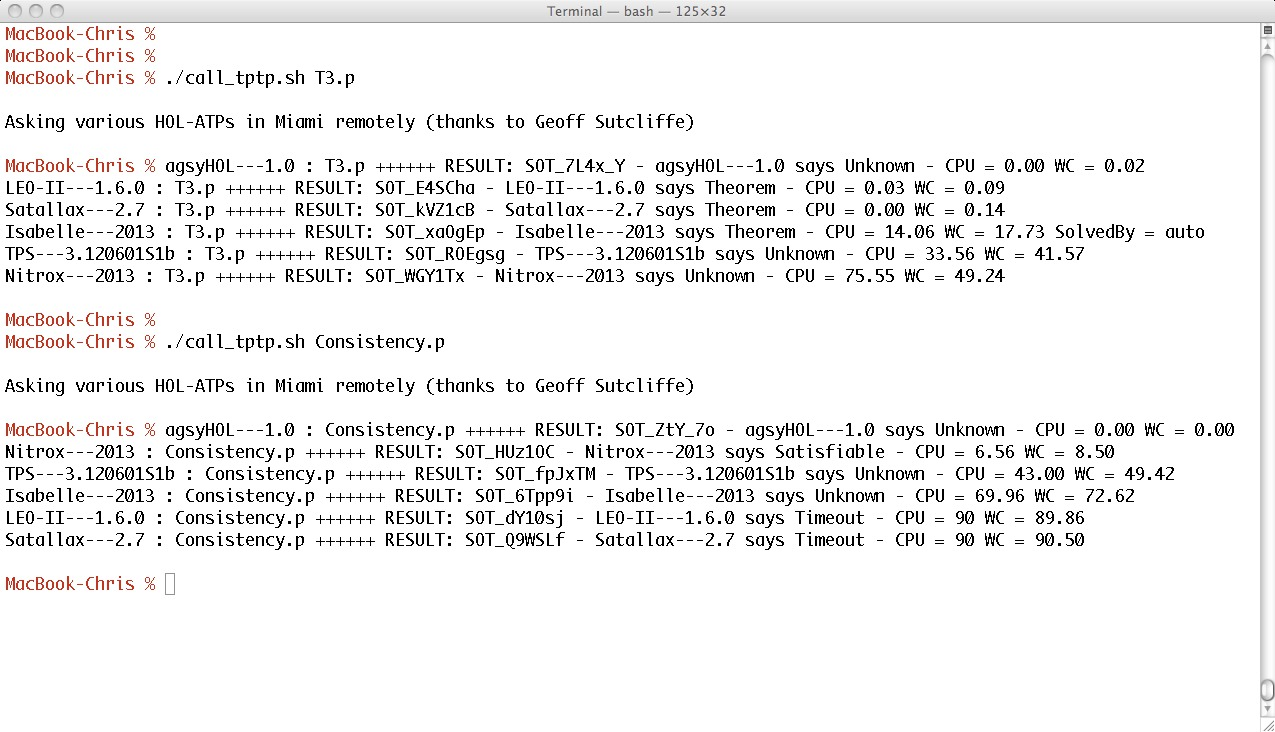
\includegraphics[width=\textwidth]{Images/Demos/DemoGrap}} 
\vfill 
Provers are called remotely in Miami --- no local installation needed!
\end{frame}

\begin{frame}{Automation \& Verification in Proof Assistant
    \textsc{Isabelle/HOL}} \large
\colorbox{gray}{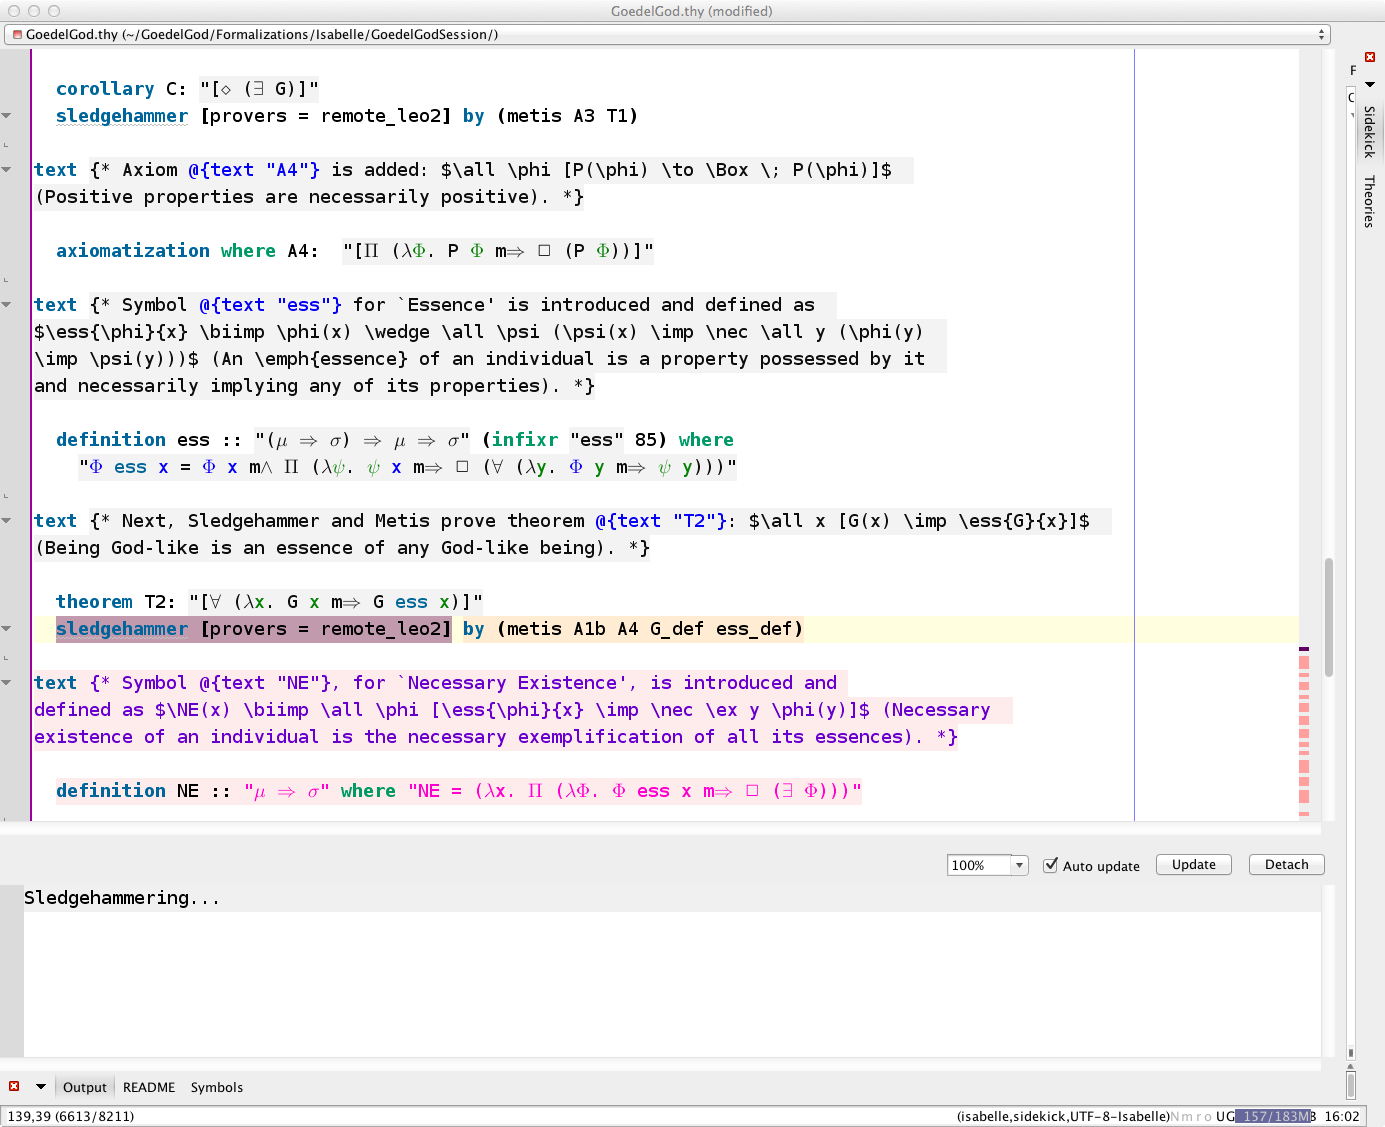
\includegraphics[width=.92\textwidth]{Images/Demos/IsabelleDemoGrab}} 
\end{frame}

\begin{frame}{Results}
\begin{changemargin}{-0.8cm}{-1.1cm}
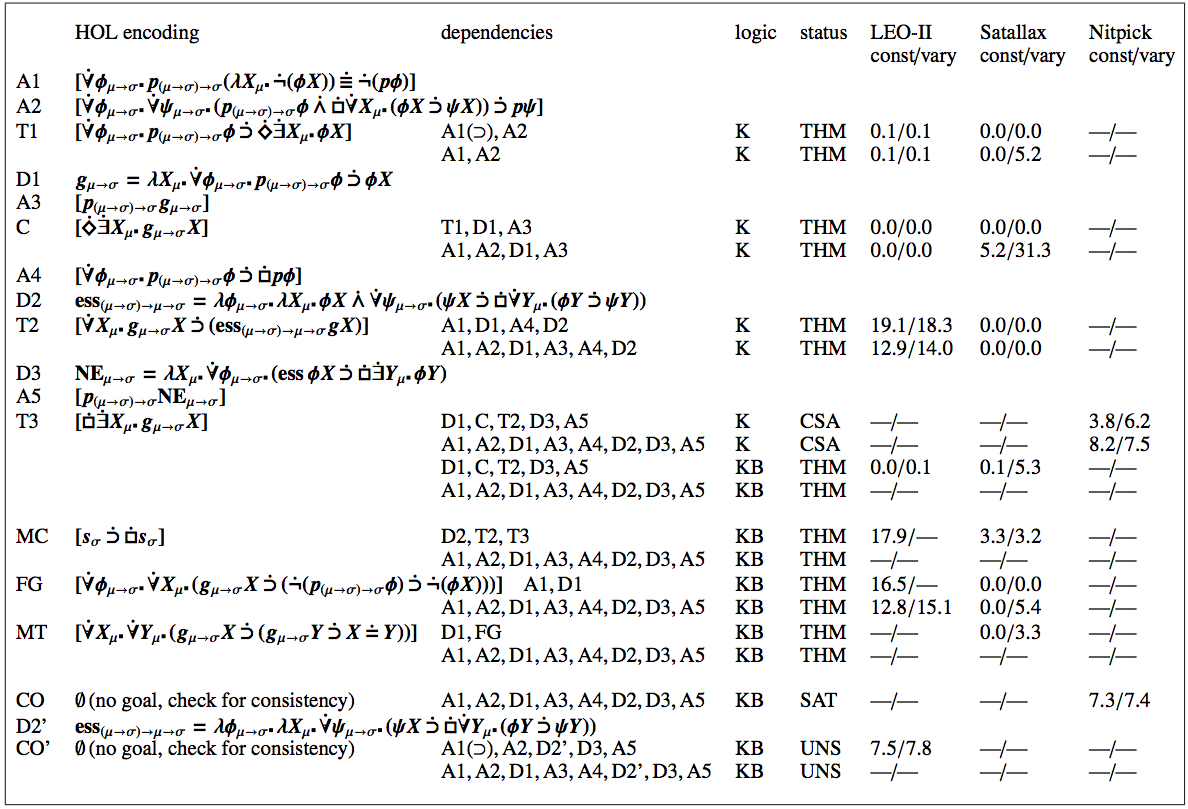
\includegraphics[width=12.4cm]{Images/Results.png}
\end{changemargin}
\end{frame}
